% Created 2021-11-17 Wed 00:12
% Intended LaTeX compiler: pdflatex
\documentclass[11pt]{article}
\usepackage[utf8]{inputenc}
\usepackage[T1]{fontenc}
\usepackage{graphicx}
\usepackage{grffile}
\usepackage{longtable}
\usepackage{wrapfig}
\usepackage{rotating}
\usepackage[normalem]{ulem}
\usepackage{amsmath}
\usepackage{textcomp}
\usepackage{amssymb}
\usepackage{capt-of}
\usepackage{hyperref}
\usepackage{minted}
\usemintedstyle{emacs}
\author{Joshua W. Brook}
\date{\today}
\title{Assignment 3: Unhealthy Conversations}
\hypersetup{
 pdfauthor={Joshua W. Brook},
 pdftitle={Assignment 3: Unhealthy Conversations},
 pdfkeywords={},
 pdfsubject={},
 pdfcreator={Emacs 26.3 (Org mode 9.1.9)}, 
 pdflang={English}}
\begin{document}

\maketitle

\section{What Makes an Comment Unhealthy?}
\label{sec:org7e9ede8}

In order to understand and identify what constitutes unhealthy online interactions, a team of researchers compiled The Unhealthy Comments Corpus (UCC).
The UCC consists of 44355 comments which have been taken from online news and media platforms, and have been meticulously classified by humans. 
These are the labels which subjects were asked to assign to each comment in the corpus:

\begin{itemize}
\item antagonistic
\item condescending
\item dismissive
\item generalisation
\item generalisation\_unfair
\item hostile
\item sarcastic
\item healthy
\end{itemize}

\noindent
These labels are encoded with values of either 1 or 0, representing booleans. 
A confidence value is also given for each label, in the range [0,1].
A machine learning algorithm can be implemented onto the data and used to predict whether the comments are \emph{healthy} or \emph{unhealthy} based on the values of the labels.


\section{Predicting Unhealthy Comments}
\label{sec:orgf1d2871}

\subsection{Exploring the Data}
\label{sec:orgee6b8f0}

The original comments are taken from the SFU Opinion and Comments Corpus (SOCC), which is compiled of comments taken from opinion articles available online.
The data is already split into three .csv files - train, test, and validation.
Each row of data has a comment, taken at random from the main dataset, as well as all associated labels and their confidence values.
The data is well structured and doesn't require any additional cleaning or formatting.


\subsection{Classifying the Data}
\label{sec:org259bc97}

I tried implementing multiple different classifiers from the scikit-learn library to see which one's could best fit the data. 
In general, ensemble methods performed much better than standard classifiers.
Following the \textbf{Scikit-Learn cheat-sheet}, I started by implementing a \textbf{KNeighbors} classifier.
This was reached as we are trying to predict a category from labelled numerical data with less than 100K samples.
Expanding on this, I implemented some ensemble methods to really try and stretch the accuracy of predictions.
Implenting \textbf{RandomForest} and \textbf{GradientBoosting} classifiers increased the accuracy, but only slightly.
I fiddled with some \emph{for loops} to check the accuracy scores for different hyperparameters of each classifier.
I finally settled on using a voting classifier based on these three classifiers (now with optimised hyperparameters) and utilising hard voting to get the best results that I could.
Strangely enough, classifying just based on the \emph{hostile} and \emph{antagonize} labels returned the best accuracy score; proving that sometimes less is indeed more.
Ideally, this data could be visualised with a nice scatter plot or some histograms, but unfortunately binary data is not very exciting to look at.
In the next section, I will implement the optimal version of my code and analyse the results.

\begin{figure}[H]
\centering
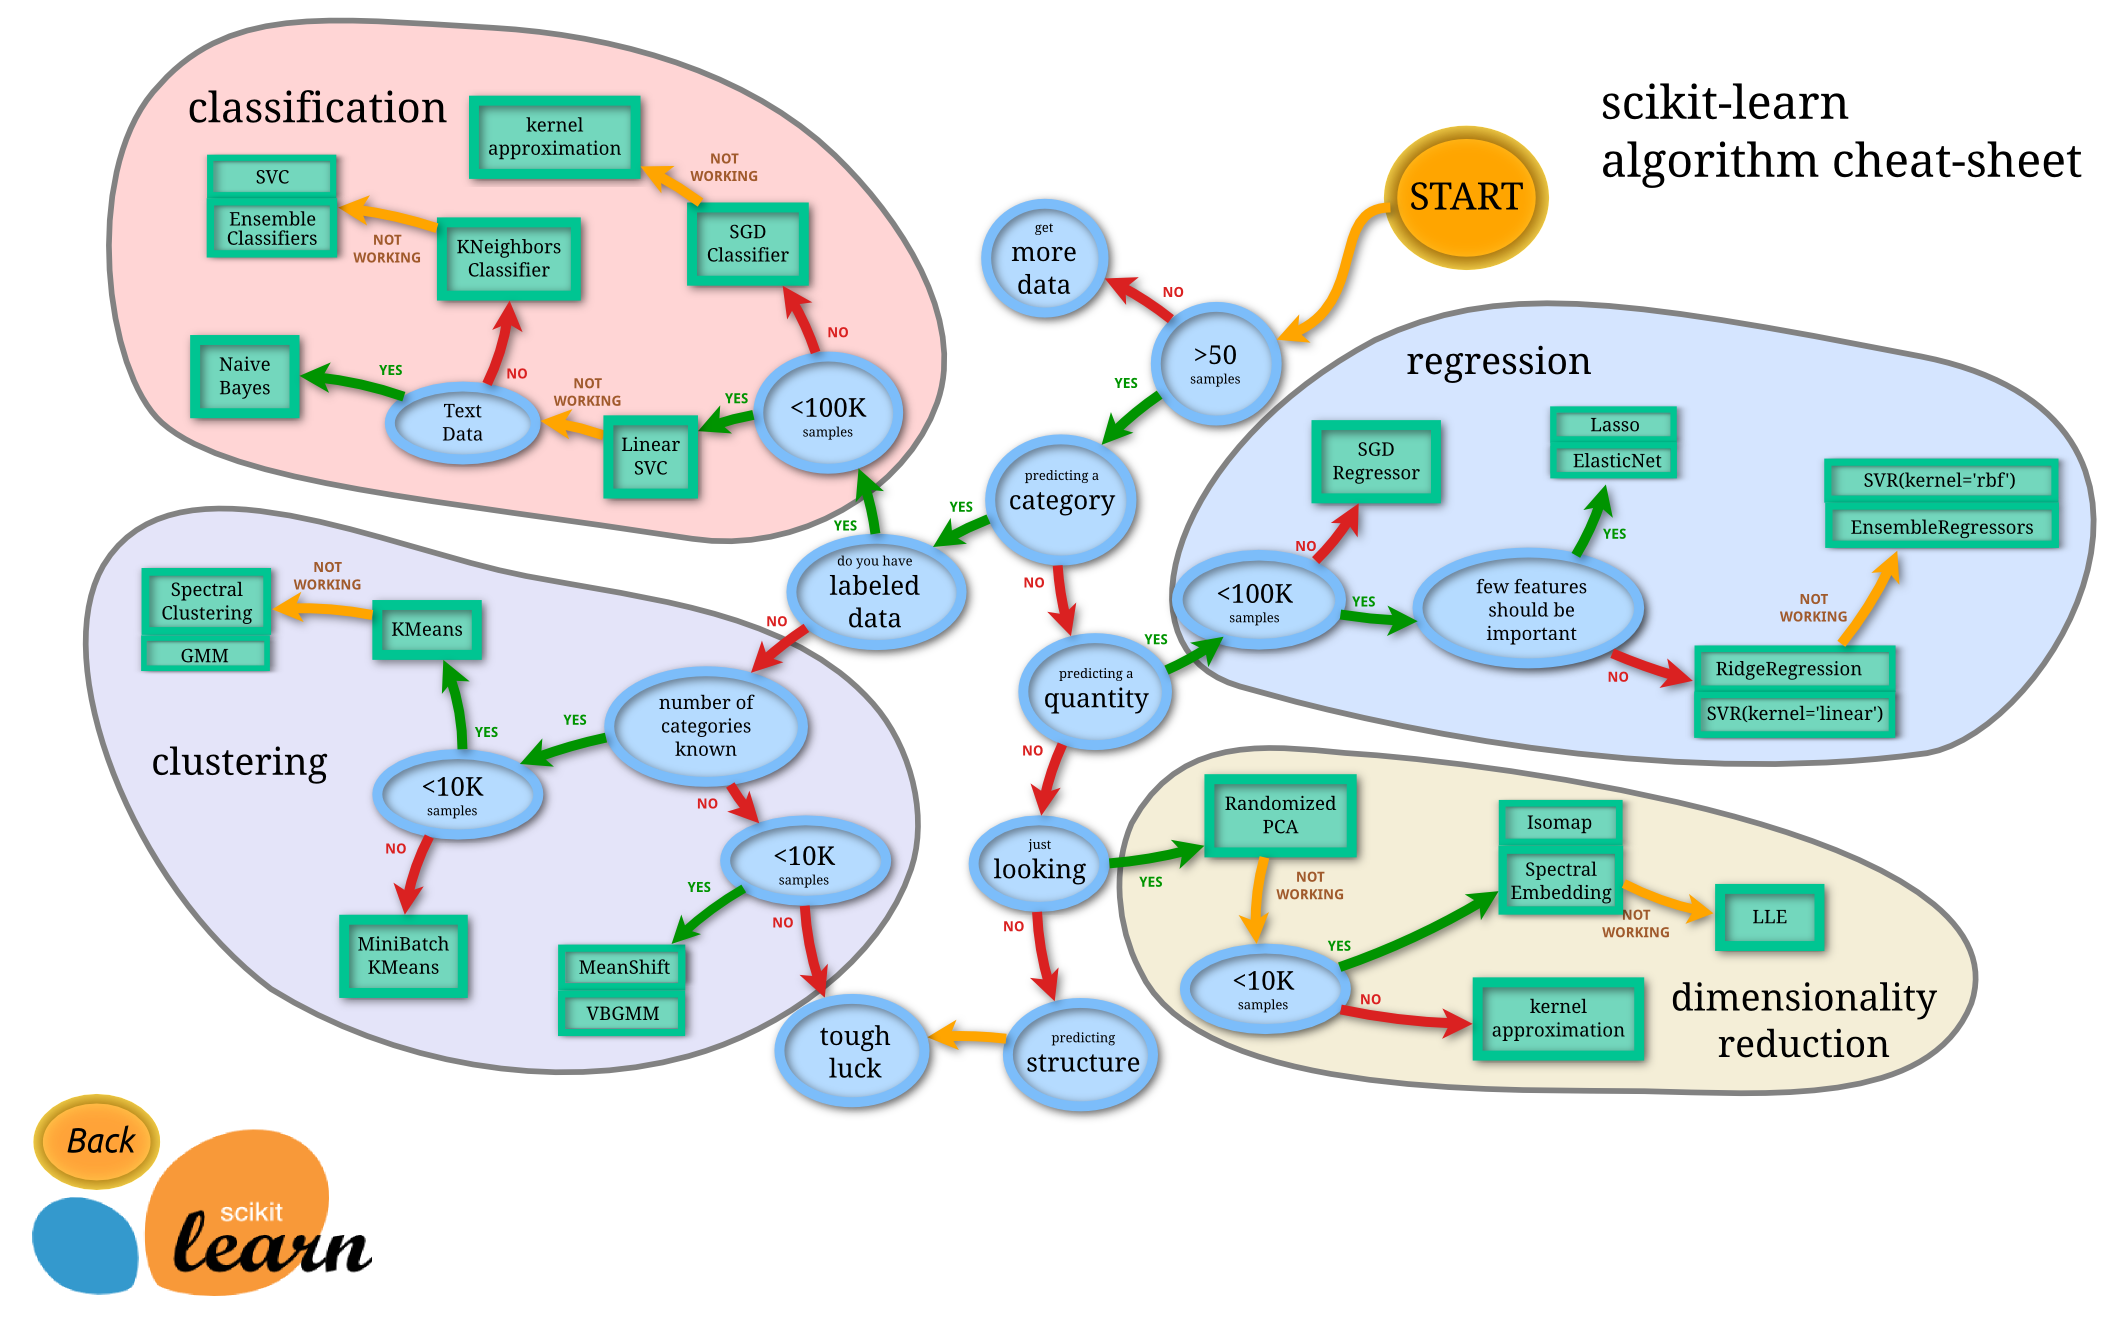
\includegraphics[width=.9\linewidth]{ml_map.png}
\caption{Sci-Kit Learn Cheat Sheet}
\end{figure}


\section{Implementation of Machine Learning}
\label{sec:orgd9af3eb}

\subsection{Importing}
\label{sec:orgb3c008e}
Let's try running some code on the UCC data to try and predict whether a comment is healthy or not.
I'll begin by doing some general imports from pandas, scikit-learn and the UCC datasets.

\begin{minted}[]{python}

import pandas as pd

from sklearn.metrics import accuracy_score
from sklearn.neighbors import KNeighborsClassifier
from sklearn.ensemble import ( GradientBoostingClassifier, 
			       VotingClassifier, 
			       RandomForestClassifier )

data = pd.read_csv("corpus/train.csv")
testdata = pd.read_csv("corpus/test.csv")

\end{minted}


\subsection{Classification}
\label{sec:org0be717c}
With these imports we can beign to classify some comments.
Let's start by grouping together the labels for ease of use, as well as defining the train and test data sets. 
I'll also set up all the classifers that I imported by defining their hyperparameters.

\begin{minted}[]{python}

all_attributes = ["antagonize" , "condescending", "dismissive", 
	      "generalisation", "generalisation_unfair", 
	      "hostile", "sarcastic"]

best_attributes = ["antagonize", "hostile"]

X = data[best_attributes]
y = data["healthy"]

Xtest = testdata[best_attributes]
ytest = testdata["healthy"]

knn = KNeighborsClassifier(n_neighbors=10)
rfc = RandomForestClassifier(n_estimators=200, random_state=42)
gbc = GradientBoostingClassifier(n_estimators=100, 
		learning_rate=1.0, max_depth=1, random_state=0)

vote = VotingClassifier(estimators=[("gbc", gbc), 
				    ("rfc", rfc),
				    ("knn", knn) ], 
			voting='hard')

\end{minted}


\subsection{Testing}
\label{sec:org2bf4512}
With the classifiers set up, we can fit the best one to the training data and finally predict which values from the test set are healthy.
I'll also add some code to print the results and an accuracy score based on the real values for \emph{healthy} vs the predictions.

\begin{minted}[]{python}

clf = vote

clf.fit(X, y)
ypred = clf.predict(Xtest)
acc = accuracy_score(ytest, ypred)

p = print("Accuracy Score:", acc,
	  "\nytest: True Values:\n", ytest.value_counts(), 
	  "\n\nypred: Predictions:\n", pd.Series(ypred).value_counts())

\end{minted}


\subsection{Results}
\label{sec:orge9ac80f}

\noindent 
Accuracy Score: 0.944858757062147\\

\noindent 
ytest: True Values:\\
1    4105\\
0     320\\
Name: healthy, dtype: int64\\

\noindent 
ypred: Predictions:\\
1    4197\\
0     228\\
dtype: int64\\


\subsection{Analysis}
\label{sec:orgcb349a2}

The values that have been assigned to the testing data by humans are shown above, under \emph{True Values}. 
As we can see, there are 4105 comments assigned as \emph{healthy} and another 320 as \emph{unhealthy}.
The classification algorithms that I implemented assign 4197 as \emph{healthy} and 228 as \emph{unhealthy}.
This gives an accuracy of 94.49\%, and if we run a bit more code on our predictions we can see which comments are incorrectly assigned.
We get 255 comments which have been incorrectly assigned in one way or another.

\begin{table}[htbp]
\centering
\begin{tabular}{rrr}
\textbf{Index} & \textbf{True} & \textbf{Predicted}\\
\hline
3 & 1.0 & 0.0\\
10 & 0.0 & 1.0\\
19 & 1.0 & 0.0\\
35 & 1.0 & 0.0\\
60 & 0.0 & 1.0\\
\ldots{} & \ldots{} & \ldots{}\\
4250 & 0.0 & 1.0\\
4269 & 0.0 & 1.0\\
4331 & 0.0 & 1.0\\
4336 & 0.0 & 1.0\\
4420 & 0.0 & 1.0\\
\end{tabular}
\caption{Incorrectly Assigned Comments}

\end{table}


\section{Plots}
\label{sec:org1ee0b7d}

\begin{figure}[H]
\centering
\includegraphics[width=.9\linewidth]{hist.png}
\caption{Histogram Plots of Label Values}
\end{figure}
\end{document}
